\scanpage{84}
% archive foliation: 83
Enfin, si $X=\bigoplus_{1\leq i\leq r}X_i$, la décomposition de $\Gamma^*(X)$ en \deleted{les} $\bigotimes\Gamma^*(X_i)$ donne \deleted{\unsure{une}} décomposition des $\unsure{\mathcal P|P}_n(\prod X_i;Y)$ en des $\unsure{\mathcal P|P}_{\nu_1,\ldots,\nu_r}(X_1,\ldots,X_r,Y)$.
On vérifie alors les axiomes c) à g), et le fait que \deleted{\unsure{il y a}} les produits tensoriels de $\unsure{\mathcal P|P}_1$ sont \uline{stricts} pour $\unsure{\mathcal P|P}$ (\unsure{vis} quelc. des facteurs), que les $\Gamma^{\nu_i}$ existent et satisfont la condition énoncée précédemment\ldots
\figure{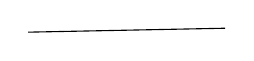
\begin{tikzpicture}\draw (0,0)--(2.5,.05);\end{tikzpicture}}
Une catégorie polynomiale $\unsure{\mathcal P|P}$ est dite \uline{stricte} si elle satisfait aux conditions préliminaires permettant de définir $\otimes$ et $\Gamma^*$ avec toutes les propriétés envisagées. D'autre part, une cat additive $\unsure{\mathcal P|P}_1$ avec $\otimes$ et $\Gamma^*$ avec les structures décrites, est dite une $\otimes$-pd-catégorie. Les deux notions sont donc en équivalence.

On dit que $\unsure{\mathcal P|P}$ est \deleted{\unsure{$k$-li}} une catégorie polynomiale (resp $\otimes$pd-cat) $k$-linéaire ($k$ anneau comm) si on a donné un hom d'anneau
\[k\longrightarrow\operatorname{End}(\mathrm{Id}_{\unsure{\mathcal P|P}_1})\quad(\unsure{\subset\mathrm{id}_\unsure{\mathcal P|P}|\in\mathrm{id}_\unsure{\mathcal P|P}}).\]

